\sect{Аналитическая часть}
\label{cha:A}
В данной части приводится анализ предметной области и формализуются данные и задачи программного обеспечения. Также приводится анализ моделей баз данных.

%=======================================================================================================================
\subsect{Анализ предметной области}
Создание парковочных мест является неотъемлемой частью организации дорожно-транспортной системы. 
Один из самых удобных способов решения этой задачи -- автоматические автопарковки~\cite{actual_autoparking}.
Использование такого типа парковок позволяет не только снизить затраты на организацию инфраструктуры парковок, но и обеспечить круглосуточный сервис для автовладельцев.

Въезд и выезд на такие парковки осуществляется при помощи талонов или  RFID-карт. Оплачивается же время парковки на специальных устройствах~--~паркоматах, поддерживающих оплату как наличными, так и банковской картой.

Как правило, на въезде на парковку стоит табло с указанием количества свободных мест. На самой парковки ведется видеонаблюдение, что повышает безопасность припаркованного транспорта.

%=======================================================================================================================
\subsect{Анализ существующих решений}
Разработка приложения для сети автопарковок позволяет сделать процесс парковки более удобным.
В частности, с помощью приложения возможно организовать бронь парковочного места, получить информацию о количестве свободных мест, оформить абонемент, оплатить время парковки с помощью QR-кода.
Используя перечисленные возможности как критерии, был проведен анализ существующих решений, таких как: 
\begin{itemize}
	\item Came Vector~\cite{came_vector};
	\item Квазар~\cite{kvazar};
	\item Московский паркинг~\cite{parking_Moscow}.
\end{itemize}
Результаты анализа приведены в таблице~\ref{tab:existing_decision}.

\renewcommand{\thetable}{\thesubsection.\arabic{table}}
\begin{table}[H]
	\begin{center}
		\begin{center}
			\caption{\label{tab:existing_decision}Сравнение известных решений}
		\end{center}
		\begin{tabular}{|c|c|c|c|}
			\hline 
			~ & Московский паркинг & Came Vector & Квазар \\ \hline
        Возможность брони & нет & нет & нет \\ \hline
        \specialcell{Информация о количестве \\ свободных мест} & да & да & нет \\ \hline
        Оформление абонемента & да & нет & да \\ \hline
        Оплата с помощью QR-кода & нет & нет & нет \\ \hline
		\end{tabular}
	\end{center}
\end{table}
Как видно из результатов анализа, ни одно из существующих решений не удовлетворяет всем решениям.

%=======================================================================================================================
\subsect{Формализация задача}
В рамках курсовой работы необходимо разработать базу данных для хранения информации о парковках и приложение для получения и обработки информации, хранящейся в ней.
В приложении необходимо реализовать следующих акторов: пользователь, гость (незарегистрированный пользователь), администратор парковки, паркомат (устройство для фиксации начала и окончания парковки).
Диаграмма использования приложения приведена на рисунке~\ref{fig:use_case}.
\renewcommand{\thefigure}{\thesubsection.\arabic{figure}}
\begin{figure}[h]
	\centering
	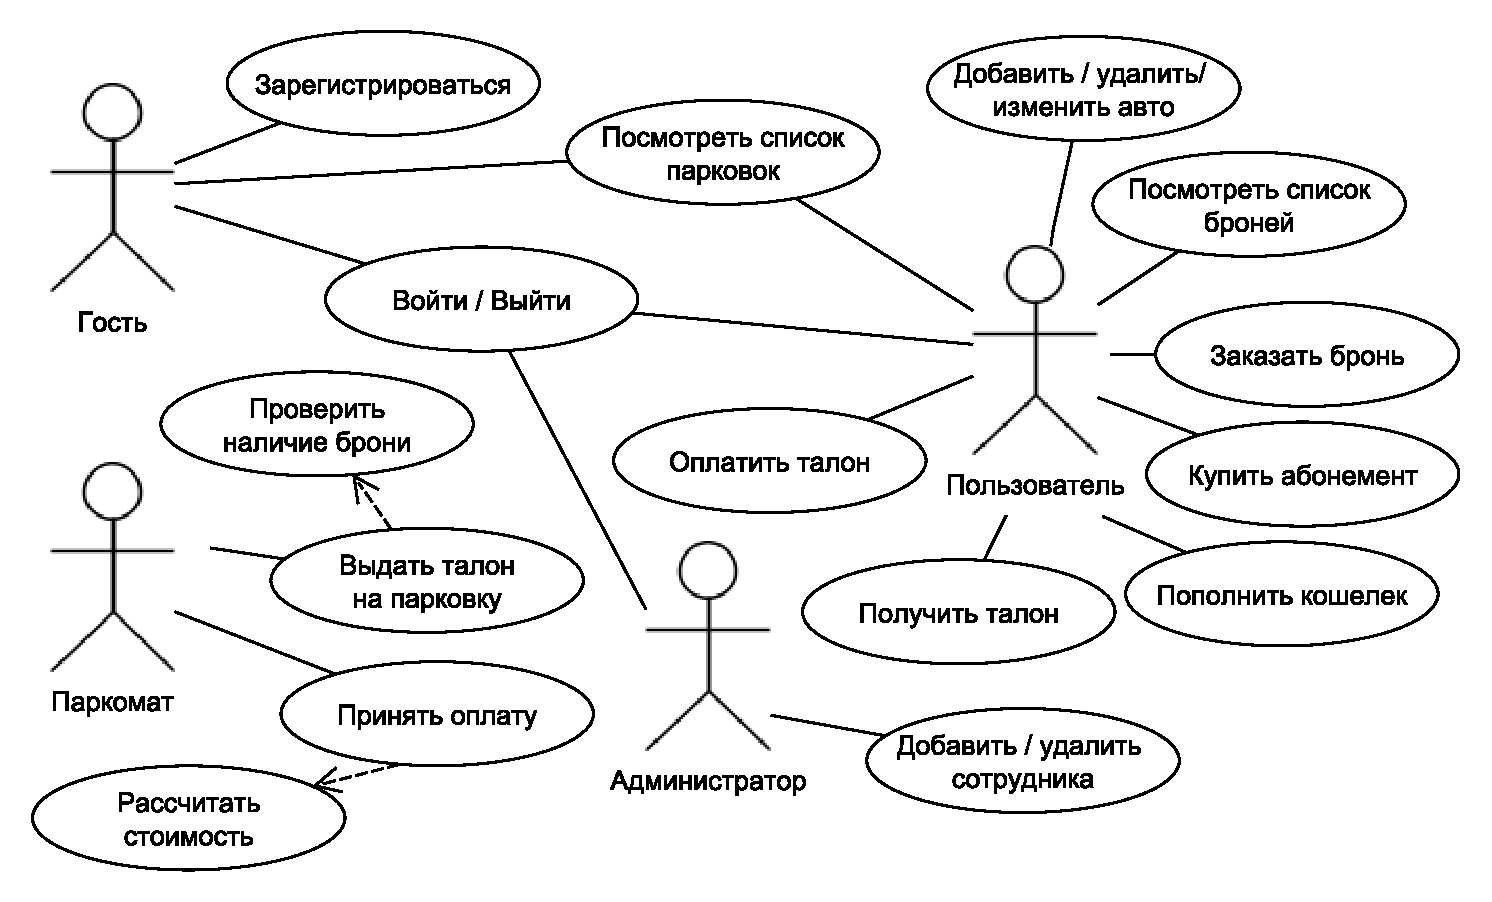
\includegraphics[height=0.35\textheight]{svg/use_case}
	\caption{Диаграмма использования приложения}
	\label{fig:use_case}
\end{figure}

%=======================================================================================================================
\subsect{Формализация данных}
В результате анализа предметной области и формализации задачи был сформирован набор сущностей.
Информация о них представлена в таблице~\ref{tab:ER}.

\begin{table}[H]
	\begin{center}
		\begin{center}
			\caption{\label{tab:ER}Сущности базы данных}
		\end{center}
		\begin{tabular}{|c|p{10cm}|}
			\hline 
			Сущность & Атрибуты \\ \hline
        Парковка & Адрес, количество мест (всего и свободных), действующий тариф  \\ \hline
        Автовладелец & ФИО, текущий абонемент, состояние счета \\ \hline
        Бронь & Статус, даты начала и окончания, автовладелец, парковка \\ \hline
        Парковочный талон & Статус, даты начала и окончания, автовладелец, парковка \\ \hline
        Транспорт & Номер, марка \\ \hline
        Абонемент & Название, стоимость, срок действия, бонусы \\ \hline
        Тариф & Название, цена \\ \hline
        Паркомат & Парковка, номер въезда / выезда \\ \hline
        Сотрудник & ФИО, должность \\ \hline
        Должность & Наименование, оклад \\ \hline
		\end{tabular}
	\end{center}
\end{table}

На рисунке~\ref{fig:ER_chen} приведена ER-диаграмма сущностей в нотации Чена.
\begin{figure}[h]
	\centering
	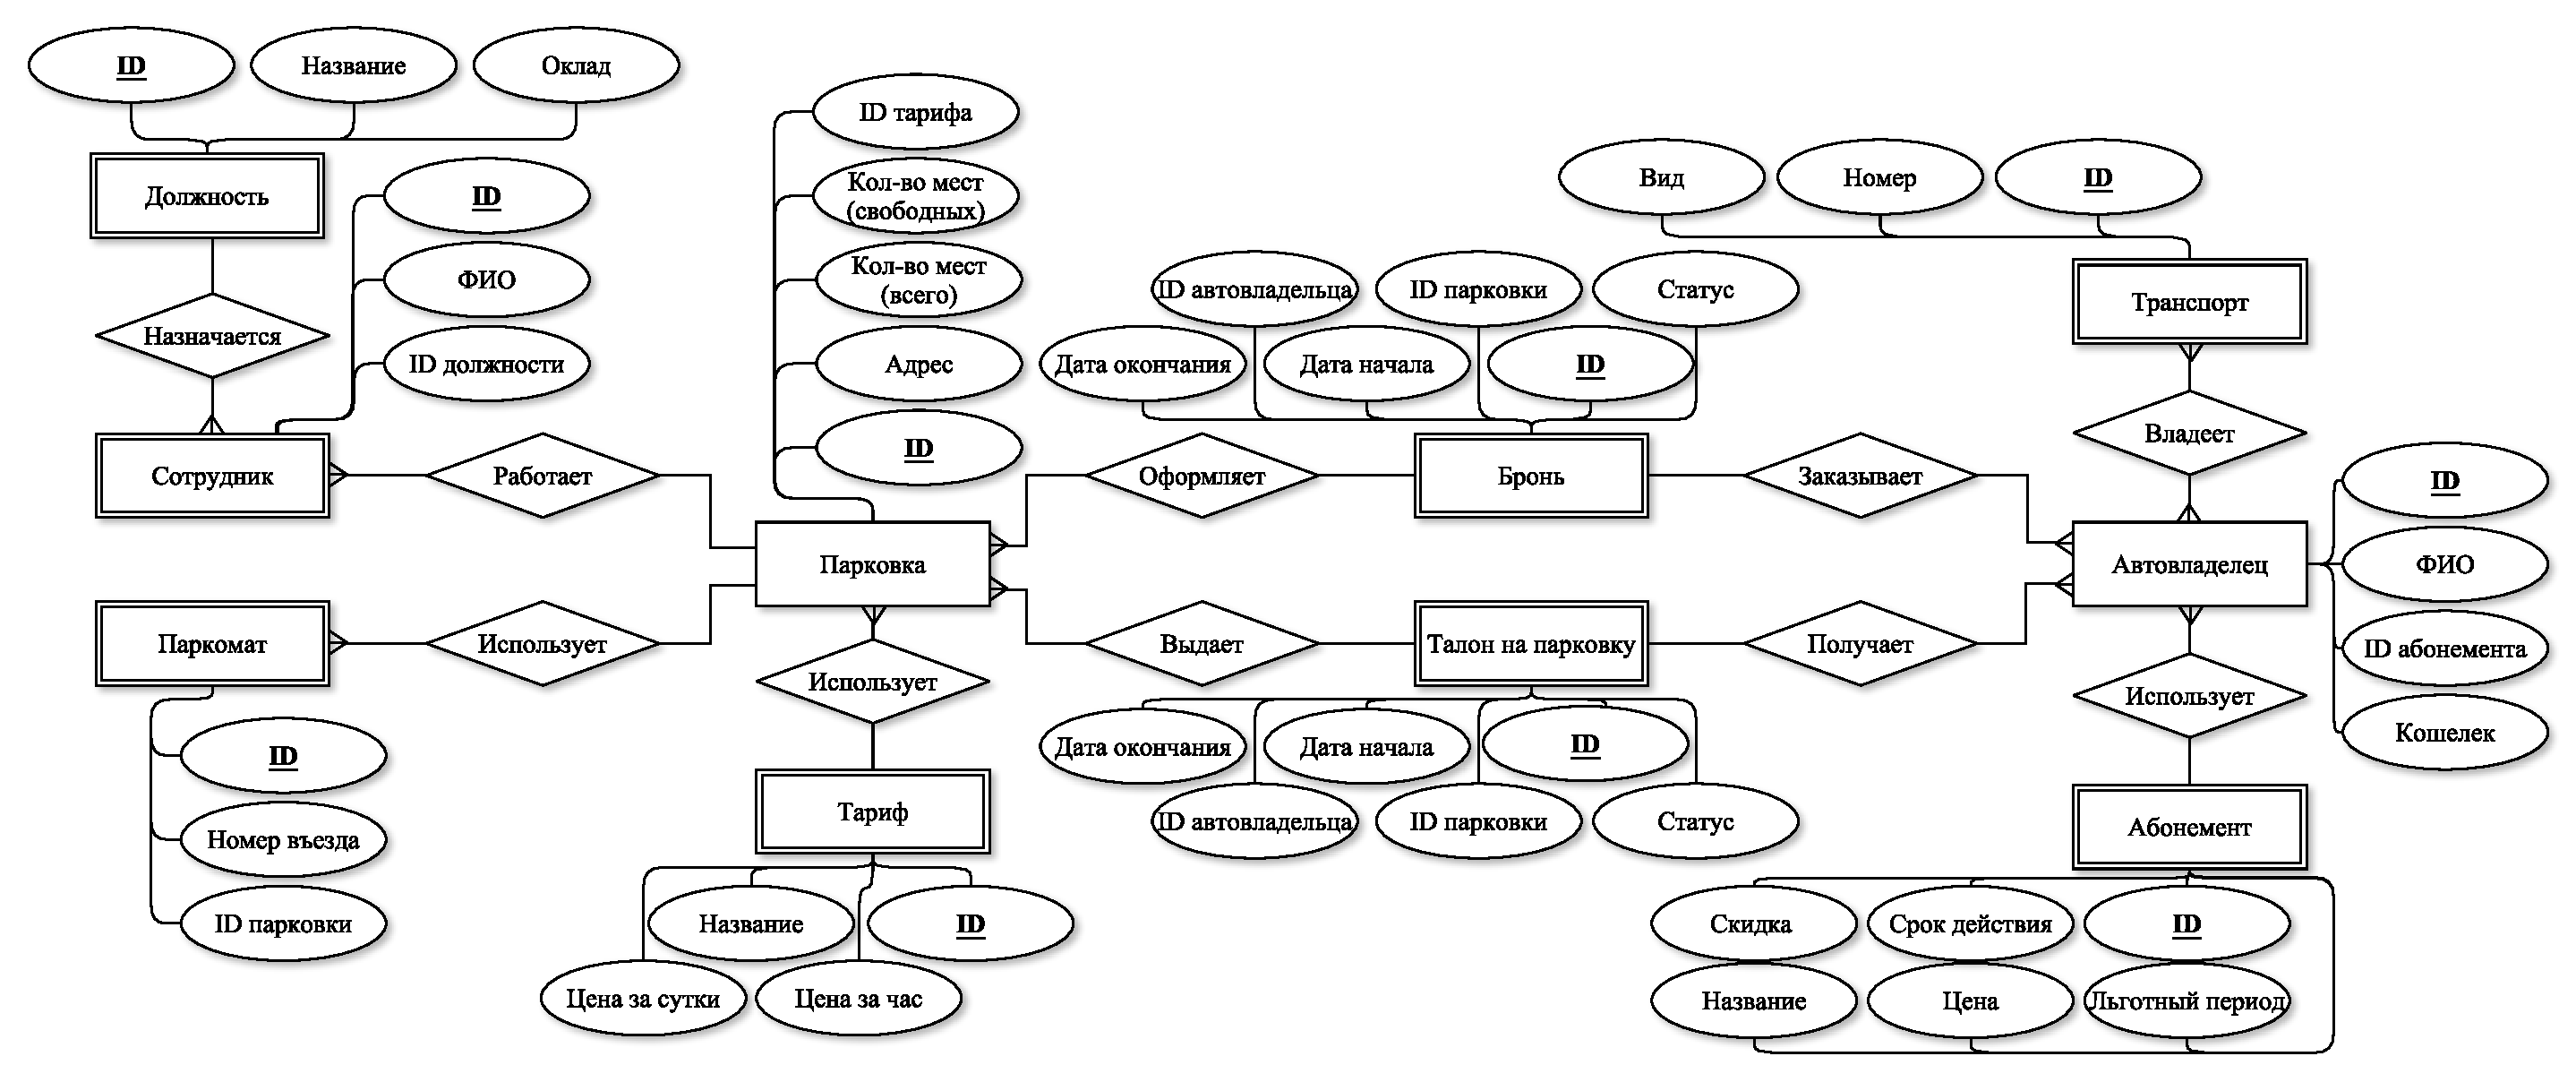
\includegraphics[height=0.5\textheight, width=1.4\textwidth, angle=90]{svg/ER_chen}
	\caption{ER-диаграмма сущностей в нотации Чена}
	\label{fig:ER_chen}
\end{figure}

%=======================================================================================================================
\subsect{Анализ баз данных}
База данных~--~это некоторый набор перманентных данных, используемых прикладными программными системами какого-либо предприятия~\cite{intro-db-williams}.

По модели хранения базы данных делятся на три группы:
\begin{itemize}
	\item дореляционные
	\item реляционные
	\item постреляционные.
\end{itemize}

\paragraph{Дореляционные базы данных}
~\par
Дореляционные модели близки к управлению данными во внешней памяти на низком уровне, 
что приводит к наилучшему использованию памяти, но такие модели данных имеют сложность  использования. 
Так как логика процедуры выбора данных зависит от физической организации этих данных, то данная модель не является полностью независимой от приложения и как следствие приводит к усложнению действий изменений в базе данных~\cite{kuznecov-db}.

\paragraph{Реляционные базы данных}
~\par
Данные реляционных баз хранятся в виде таблиц, которые могут иметь связи с другими таблицами через внешние ключи, таким образом образуя отношения~\cite{kuznecov-db}.

Структура реляционных баз данных позволяет связывать информацию из разных таблиц с помощью внешних ключей, которые используются для уникальной идентификации любого атомарного фрагмента данных в этой таблице. 
Другие таблицы могут ссылаться на этот внешний ключ.

\paragraph{Постреляционные базы данных}
~\par
Классическая реляционная модель предполагает неделимость данных, хранящихся в полях записей таблиц. 
Это означает, что информация в таблице представляется в первой нормальной форме. 
Существует ряд случаев, когда это ограничение мешает эффективной реализации приложений. 
Постреляционная база данных использует трехмерные структуры, позволяя хранить в полях таблицы другие таблицы, расширяя таким образом возможности по описанию сложных объектов реального мира~\cite{postsql-db}.

%=======================================================================================================================
\subsect{Вывод}
В данном разделе был проведен анализ предметной области и существующих, формализованы задача и используемые данные.
Также был проведен анализ баз данных, в результате которого было решено использовать реляционную базу данных.
Такой выбор обусловлен необходимостью использования разнообразных запросов различной сложности.
